\documentclass[unknownkeysallowed, 10pt, a4 paper, handout]{beamer}

% Custom beamer theme
\usepackage{../style/beamerthemeCustom}
\newcommand{\HRule}{\rule{\linewidth}{0.5mm}}   %FOR TITLEPAGE

\usepackage{changepage}       % adjustwidth

\setlength\parskip{0.3cm}

\newcommand{\focus}[1]{\textbf{\textcolor{red}{#1}}}
\newcommand{\ra}{$\longrightarrow$ }
\newcommand{\lra}{$\longleftrightarrow$ }

\newcommand{\code}[1]{\colorbox{black}{\color{green}\texttt{#1}}}

% Command to create two side-by-side minipages
\newcommand{\sidebyside}[5]{
  \begin{minipage}{#1\textwidth}
    #2
  \end{minipage} #3 \begin{minipage}{#4\textwidth}
    #5
  \end{minipage}
}

\begin{document}

\begin{frame}
  \begin{center}

    \definecolor{myblue}{RGB}{51,51,179}
    \setbeamercolor{block body}{use=structure,fg=white,bg=myblue!20!myblue}

    \begin{block}{}
      \Large
      \centering
      Linux Basics I:\\
      What is Linux, the filesystem
    \end{block}

    \vspace{6mm}
    \large
    \textsc{Adriano Angelone, Graziano Giuliani} \\

  \end{center}
\end{frame}


\begin{frame}[label=outline]{Course Outline}
  \begin{itemize}
    \item UNIX/Linux Basics
    \item Intermediate shell commands
    \item Editing and compiling source code
    \item Text file manipulation
    \item Basic shell scripting
  \end{itemize}

  \vspace{6mm}

  \centering
  Download slides and exercise files with the command\\
  \code{git clone https://github.com/AA24KK/LinuxBasics.git}\\
  \vspace{1mm}
  or download a ZIP archive at
  \vspace{1mm}
  \code{https://github.com/AA24KK/LinuxBasics/archive/master.zip}

  \vspace{2mm}

  Adriano: \focus{aangelon@ictp.it}, Room 263, ICTP\\
  Graziano: \focus{ggiulian@ictp.it}

\end{frame}


\begin{frame}[label=pdp11]{The Origin of the OS}
  \begin{center}
    \includegraphics[scale=3.5]{pics/pdp11.jpg}
  \end{center}
  \begin{flushright}
    \tiny{By Peter Hamer - Ken Thompson (sitting) and Dennis Ritchie at
    PDP-11 Magnus Manske, CC BY-SA 2.0}
  \end{flushright}
\end{frame}


\begin{frame}[label=unix]{UNIX Philosophy}
  \begin{enumerate}
    \item Make each program do one thing well. %To do a new job, build
      % afresh rather than complicate old programs by adding new "features".
    \item Expect the output of every program to become the input to another.
      %, as yet unknown, program. Don't clutter output with extraneous
      % information. Avoid stringently columnar or binary input formats.
      % Don't insist on interactive input.
    % \item Design and build software, even operating systems, to be tried
      % early, ideally within weeks. Don't hesitate to throw away the clumsy
      % parts and rebuild them.
    % \item Use tools in preference to unskilled help to lighten a programming
      % task, even if you have to detour to build the tools and expect to
      % throw some of them out after you've finished using them.
    % \item Write programs to handle text streams, because that is a
      % universal interface.
    \item Purpose of computation is data transformation
  \end{enumerate}
  \vfill
  \emph{$\dots$ at its heart is the idea that the power of a system comes
  more from the relationships among programs than from the programs themselves.
  Many UNIX programs do quite trivial things in isolation, but, combined with
  other programs, become general and useful tools. \dots}
  \newline
  \begin{flushright}
  \tiny{The UNIX Programming Environment, Brian Kernighan and Rob Pike, 1984}
  \end{flushright}
\end{frame}


\begin{frame}[label=os]{The Linux OS - UNIX free}
  \begin{center}
    \includegraphics[scale=0.5]{pics/linux-first-announcement-email.png}
  \end{center}
\end{frame}


\begin{frame}[label=gnu]{The Free Software Movement}
  Free Software is not just Open Source or Gratis % Latin : as a kindness
  \begin{columns}[T]
    \begin{column}{.65\textwidth}
      \begin{itemize}
        \item The freedom to run the program as you wish, for any purpose.
        \item The freedom to study how the program works, and change it so it
          does your computing as you wish
        \item The freedom to redistribute copies so you can help others
        \item The freedom to distribute copies of your modified versions
          to others
      \end{itemize}
    \end{column}
    \hfill
    \begin{column}{.32\textwidth}
      \includegraphics[scale=0.45]{pics/rms1.png}
    \end{column}
  \end{columns}
\end{frame}


\begin{frame}[label=architecture]{UNIX architecture}
  \begin{columns}[T]
    \begin{column}{.23\textwidth}
      \includegraphics[scale=0.5]{pics/UNIX-HATERS_Handbook_cover_ISBN_1-56884-203-1.png}
    \end{column}
    \begin{column}{.73\textwidth}
      \begin{itemize}
      \item The kernel is a program, running in supervisor mode, that acts as a
        program loader and supervisor for the user programs providing locking
        and I/O services.
      \item The system services or daemons are programs running on the system
        and providing facilities that allow or enhance access to system
        resources
      \item User programs are task controlled interactively or through batch job
        submission system by physical user concurrently accessing system
        resources through multi tasking sharing the CPU(s).
    \end{itemize}
    \end{column}
  \end{columns}
\end{frame}


%\begin{frame}[label=file]{Everything is a file (descriptor)}
%  All input/output resources such as documents, directories, hard-drives,
%  screens, keyboards, printers and even some inter-process and network
%  communications are simple streams of bytes exposed through the
%  filesystem name space.
%  \begin{itemize}
%    \item There are a number of file types.
%    \item When a file is opened, a file descriptor is created. The file path
%      becoming the addressing system and the file descriptor being the byte
%      stream I/O interface.
%    \item Different methods are used to create file descriptors for things
%      like anonymous pipes and network sockets.
%    \item Pseudo and virtual filesystems exists which exposes information
%      about processes and other system information in a hierarchical file-like
%      structure.
%  \end{itemize}
%\end{frame}


\begin{frame}[c]
  \begin{center}
    \frametitle{The Command Line}

    \sidebyside{0.54}{
      \focus{Graphical User Interfaces (GUI)}:\\
      comfortable, sometimes lack flexibility
    }{\hfill}{0.41}{
      \includegraphics[width=\textwidth]{pics/gui.png}
    }

    \sidebyside{0.54}{
      \focus{Command Line Interface (CLI)}:\\
      powerful, requires knowledge
    }{\hfill}{0.41}{
      \includegraphics[width=\textwidth]{pics/cli.png}
    }

    \vspace{-2mm}

    We're here to learn (mostly) how to use CLI:\\
    headaches at first, more productivity in the end

  \end{center}
\end{frame}


\begin{frame}[label=login]{Authentication}
  \begin{columns}[T]
    \begin{column}{.23\textwidth}
      \begin{center}
        \includegraphics[scale=0.25]{pics/locks.png}
      \end{center}
    \end{column}
    \hfill
    \begin{column}{.66\textwidth}
    \small{
      The CLI is THE interface to a UNIX system. To reach the command
      interpreter a standard procedure is used:
      \begin{itemize}
        \item \textbf{Authentication}: The user is authenticated with
          username/password challenge by a login program.
        \item \textbf{Authorization}: The system creates an environment
          by providing the set of system resources the user may access 
        \item \textbf{Allocation}: The user access the resources by
          running programs through the command interpreter.
      \end{itemize}
      }
    \end{column}
  \end{columns}
\end{frame}


\begin{frame}[label=shell]{The command shell}
  \begin{columns}[T]
    \begin{column}{.56\textwidth}
    \small{
      The SHELL is is the command interpreter:
      \begin{itemize}
        \item waits for the user command input showing up a prompt 
        \item controls the user environment through variables
        \item executes user commands managing the input, output
                 and error streams
      \end{itemize}
      }
    \end{column}
    \hfill
    \begin{column}{.43\textwidth}
      \begin{center}
        \includegraphics[scale=0.4]{pics/vt100.png}
      \end{center}
    \end{column}
  \end{columns}
  \begin{center}
    There is not just a single shell program!
  \end{center}
\end{frame}

\begin{frame}[label=program]{The Program}
  \begin{columns}[T]
    \begin{column}{.23\textwidth}
      \includegraphics[scale=0.15]{pics/running.jpg}
    \end{column}
    \hfill
    \begin{column}{.73\textwidth}
      \small{
      A program running in the system has:
      \begin{itemize}
        \item An executable file containing:
        \begin{itemize}
          \item The instruction for the processor
          \item The data to be processed
        \end{itemize}
        \item The User credentials to access the system resources
        \item An extendable set of system resources (CPU, Memory, Storage)
        \item The capability to load system shared executable procedures
          in the form of routines and functions in libraries.
      \end{itemize}
    }
    \end{column}
  \end{columns}
\end{frame}


\begin{frame}[label=running]{Running a program}
  \begin{columns}[T]
    \begin{column}{.33\textwidth}
      \includegraphics[scale=0.99]{pics/bad_arguments.jpg}
    \end{column}
    \hfill
    \begin{column}{.63\textwidth}
      \small{
      To run a program in the shell you must know in advance:
      \begin{itemize}
        \item The program path to the executable in the file system or the
          program name if it is in a system path
        \item The options that can modify its behavior to fit your requests
        \item The type and number of arguments the program expects to
          execute
      \end{itemize}
    }
    \end{column}
  \end{columns}
  As an example, these are valid syntaxes to run a program:
  \begin{center}
  \code{ls -l Documents} \\
  \code{cp theorem.tex Documents}
  \end{center}
  \begin{center}
    \Large{What is a file path in UNIX ?}
  \end{center}
\end{frame}


\begin{frame}[c]
  \begin{center}
    \frametitle{Files, directories, exploring the filesystem}

    \focus{Files contain information, directories contain files}

    From the terminal, you \focus{navigate} the filesystem,\\
    exploring directories and opening files
    \vspace{-3mm}

    \begin{center}
      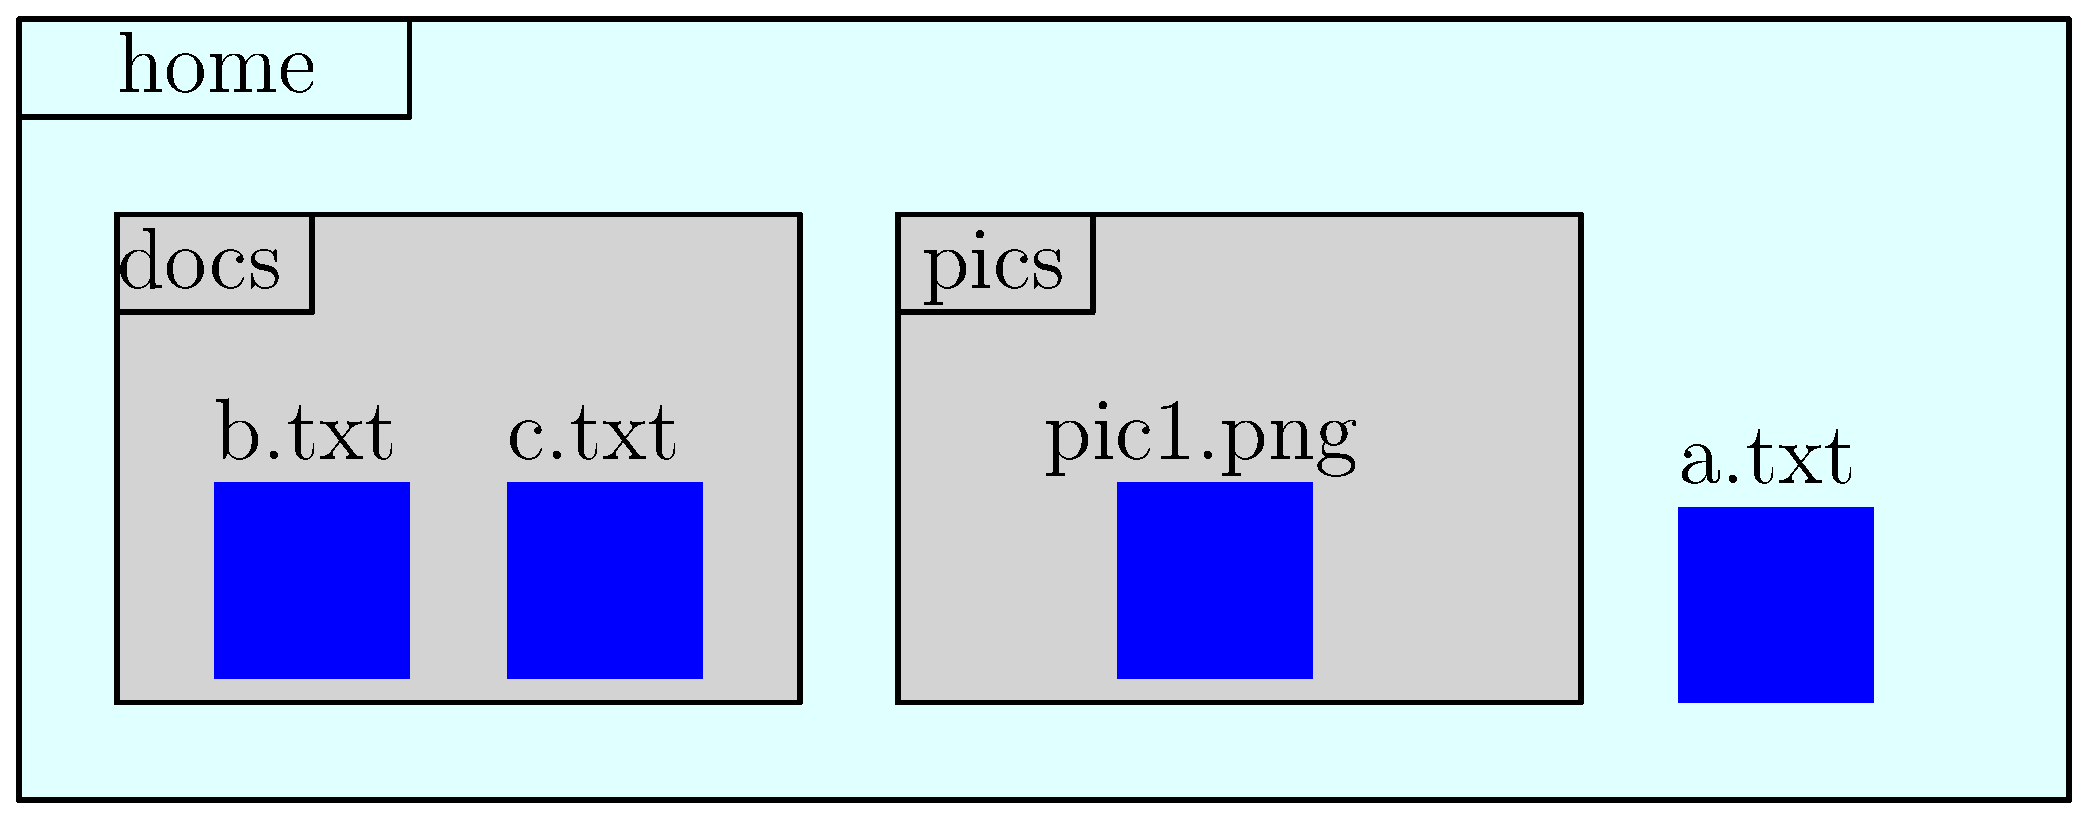
\includegraphics[width=0.90\textwidth]{pics/filesystem.eps}
    \end{center}
    \vspace{-3mm}

    Files and directories have a \focus{path} in the filesystem\\
    (for instance, \code{/home/docs/c.txt})

    Directories in a path are separated by \code{/}\\
    directory names can end in \code{/}, files can have an extension
	  (e.g., \code{.txt})

  \end{center}
\end{frame}


\begin{frame}[label=filesystem]{The file system}
  \begin{columns}[T]
    \begin{column}{.23\textwidth}
      \includegraphics[scale=0.29]{pics/fs.png}
    \end{column}
    \hfill
    \begin{column}{.73\textwidth}
      \small{
      The Filesystem Hierarchy Standard (FHS) defines the directory
      structure and directory contents in Linux:
      \begin{itemize}
        \item The filesistem root is the "/" directory
        \item All files and directories appear under the root directory /,
          even if they are stored on different physical or virtual devices.
        \item bin stands for binaries and contains system executables
        \item lib stands for libraries and contains shared or static pieces of
          code which are used by running executables or to create executables
        \item tmp stands for temporary and is where scratch files are placed
        \item etc stands for etcetera and is where configuration files are
        \item home is where user files are placed
      \end{itemize}
    }
    \end{column}
  \end{columns}
\end{frame}


\begin{frame}[c]
  \frametitle{Commands I - Pathfinding}
  Let us try to run the basic programs to navigate the Filesystem:
  \begin{center}
    \vspace{2pt}

    \code{pwd}: print the current directory path
    \vspace{-4mm}

    \begin{center}
      \includegraphics[width=0.40\textwidth]{pics/pwd.png}
    \end{center}
    \vspace{4mm}

    \code{pwd} prints the \focus{global} path\\
    (path with respect to the \focus{root directory})\\
    Example: \code{/home/documents/text/a.txt}
    \vspace{4mm}

    In commands, you can mostly use the \focus{relative path}\\
    (path with respect to the \focus{current folder})\\
    Example: \code{text/a.txt} if I am in \code{/home/documents/}
  \end{center}
\end{frame}


\begin{frame}[c]
  \begin{center}
    \frametitle{Commands II - Moving around}

    \code{ls <directory>}: list the files in the given directory\\
    no argument: list current directory
    \vspace{-2mm}

    \begin{center}
      \includegraphics[width=0.40\textwidth]{pics/ls.png}
    \end{center}

    \code{cd <directory>}: move to another directory\\
    no argument: move to your home directory
    \vspace{-2mm}

    \begin{center}
      \includegraphics[width=0.40\textwidth]{pics/cd.png}
    \end{center}

    \vspace{-4mm}

    \begin{itemize}
      \item \code{cd \~} brings you to your home directory
      \item \code{.} is your current directory
      \item \code{..} is the \textit{parent} directory (the directory containing the current one)
      \item \code{cd -} brings you to the previously visited directory
    \end{itemize}
  \end{center}
\end{frame}


\begin{frame}[c]
  \begin{center}
    \frametitle{Commands III - Creating and removing}
    \code{mkdir <directories>}: create new directories
    \vspace{-4mm}

    \begin{center}
      \includegraphics[width=0.53\textwidth]{pics/mkdir.png}
    \end{center}

    \code{touch <filenames>}: create new (empty) text files
    \vspace{-4mm}

    \begin{center}
      \includegraphics[width=0.53\textwidth]{pics/touch.png}
    \end{center}

    \code{rm <filenames>}: removes files\\
    \code{rm -r <directories>}: removes directories
    \vspace{-4.5mm}

    \begin{center}
      \includegraphics[width=0.53\textwidth]{pics/rm.png}
    \end{center}
    \vspace{-2mm}
  \end{center}
\end{frame}


\begin{frame}[c]
  \begin{center}
    \frametitle{Exercise I - mkdir, rm}
    Using the commands you know, create these directories and files,\\
    and then remove them all (\focus{after showing us}):

    \begin{center}
      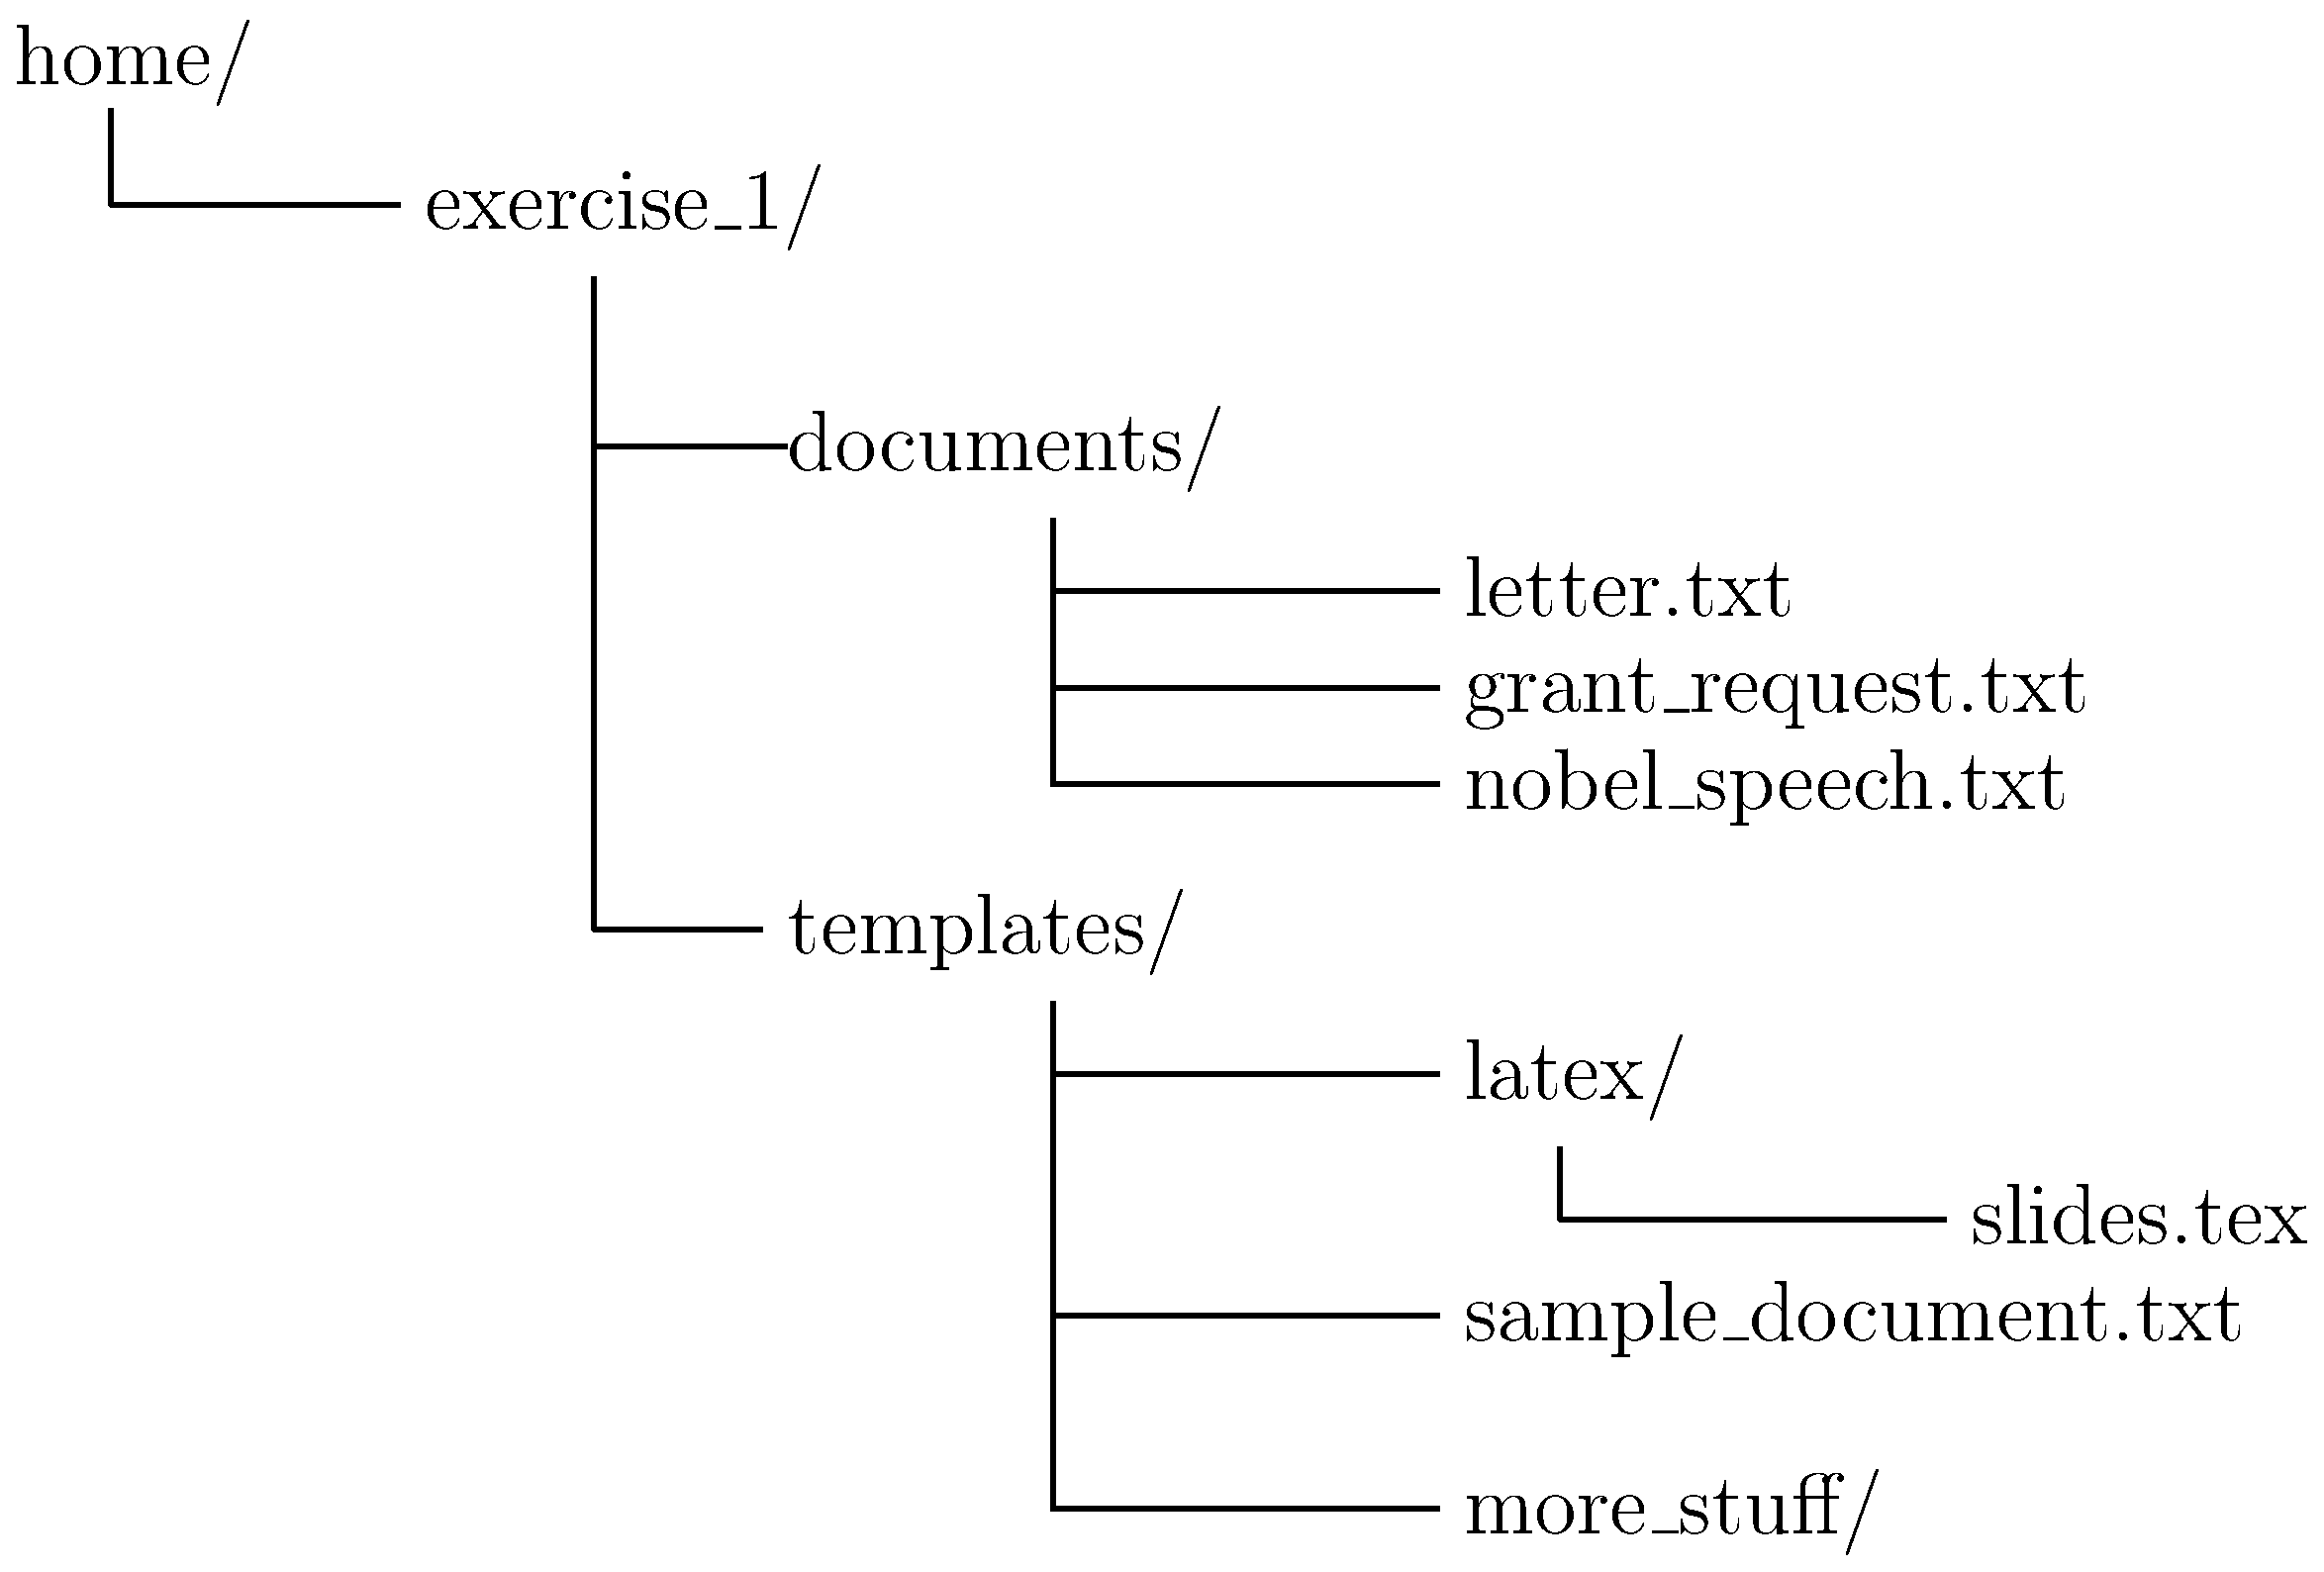
\includegraphics[width=0.80\textwidth]{pics/exercise_1.eps}
    \end{center}
  \end{center}
\end{frame}


\begin{frame}
  \begin{center}
    \frametitle{Commands IV - Moving and copying files}

    \code{cp <old\_path> <new\_path>}: \focus{copy} a file to another location\\
    \code{cp -r}: copy entire directories
    \vspace{-3mm}

    \begin{center}
      \includegraphics[width=0.50\textwidth]{pics/cp_1.png}
    \end{center}

    Paths can be relative, the copy can have a different name\\
    \vspace{-1mm}

    \begin{center}
      \includegraphics[width=0.50\textwidth]{pics/cp_2.png}
    \end{center}

    \code{<new\_path>} is overwritten, old content is lost\\
    Suggestion: use \code{cp -i}

    \code{mv}: same syntax, target \focus{moved} (old file/directory deleted)
  \end{center}
\end{frame}


\begin{frame}
  \begin{center}
    \frametitle{Commands V - Finding and listing files}

    \code{find} \focus{recursively searches files in a directory}\\
    \code{find <directory> <options>}

    \vspace{3mm}

    Many options, we will see the basic ones:

    \vspace{3mm}

    \sidebyside{0.52}{
      \begin{itemize}
        \item \code{-name}:\\
          specify file name (no paths here)
        \item \code{-path}:\\
          specify (part of) the file path
        \item \code{-printf \%\{format\}}:\\
          print details of the items found
        \item \code{-delete}:\\
          deletes the files found
      \end{itemize}
    }{\hfill}{0.45}{
      \begin{center}
        \includegraphics[width=1.00\textwidth]{pics/find.png}
      \end{center}
    }

    \vspace{3mm}

    In the above commands, you can use \focus{wildcards}:\\
    \code{*} can replace any character (more in the future)
  \end{center}
\end{frame}


\begin{frame}
  \begin{center}
    \frametitle{Exercise II - cp, mv, find}
    Using the commands you know, create these directories and files,\\
    copying and moving files as shown:

    \begin{center}
      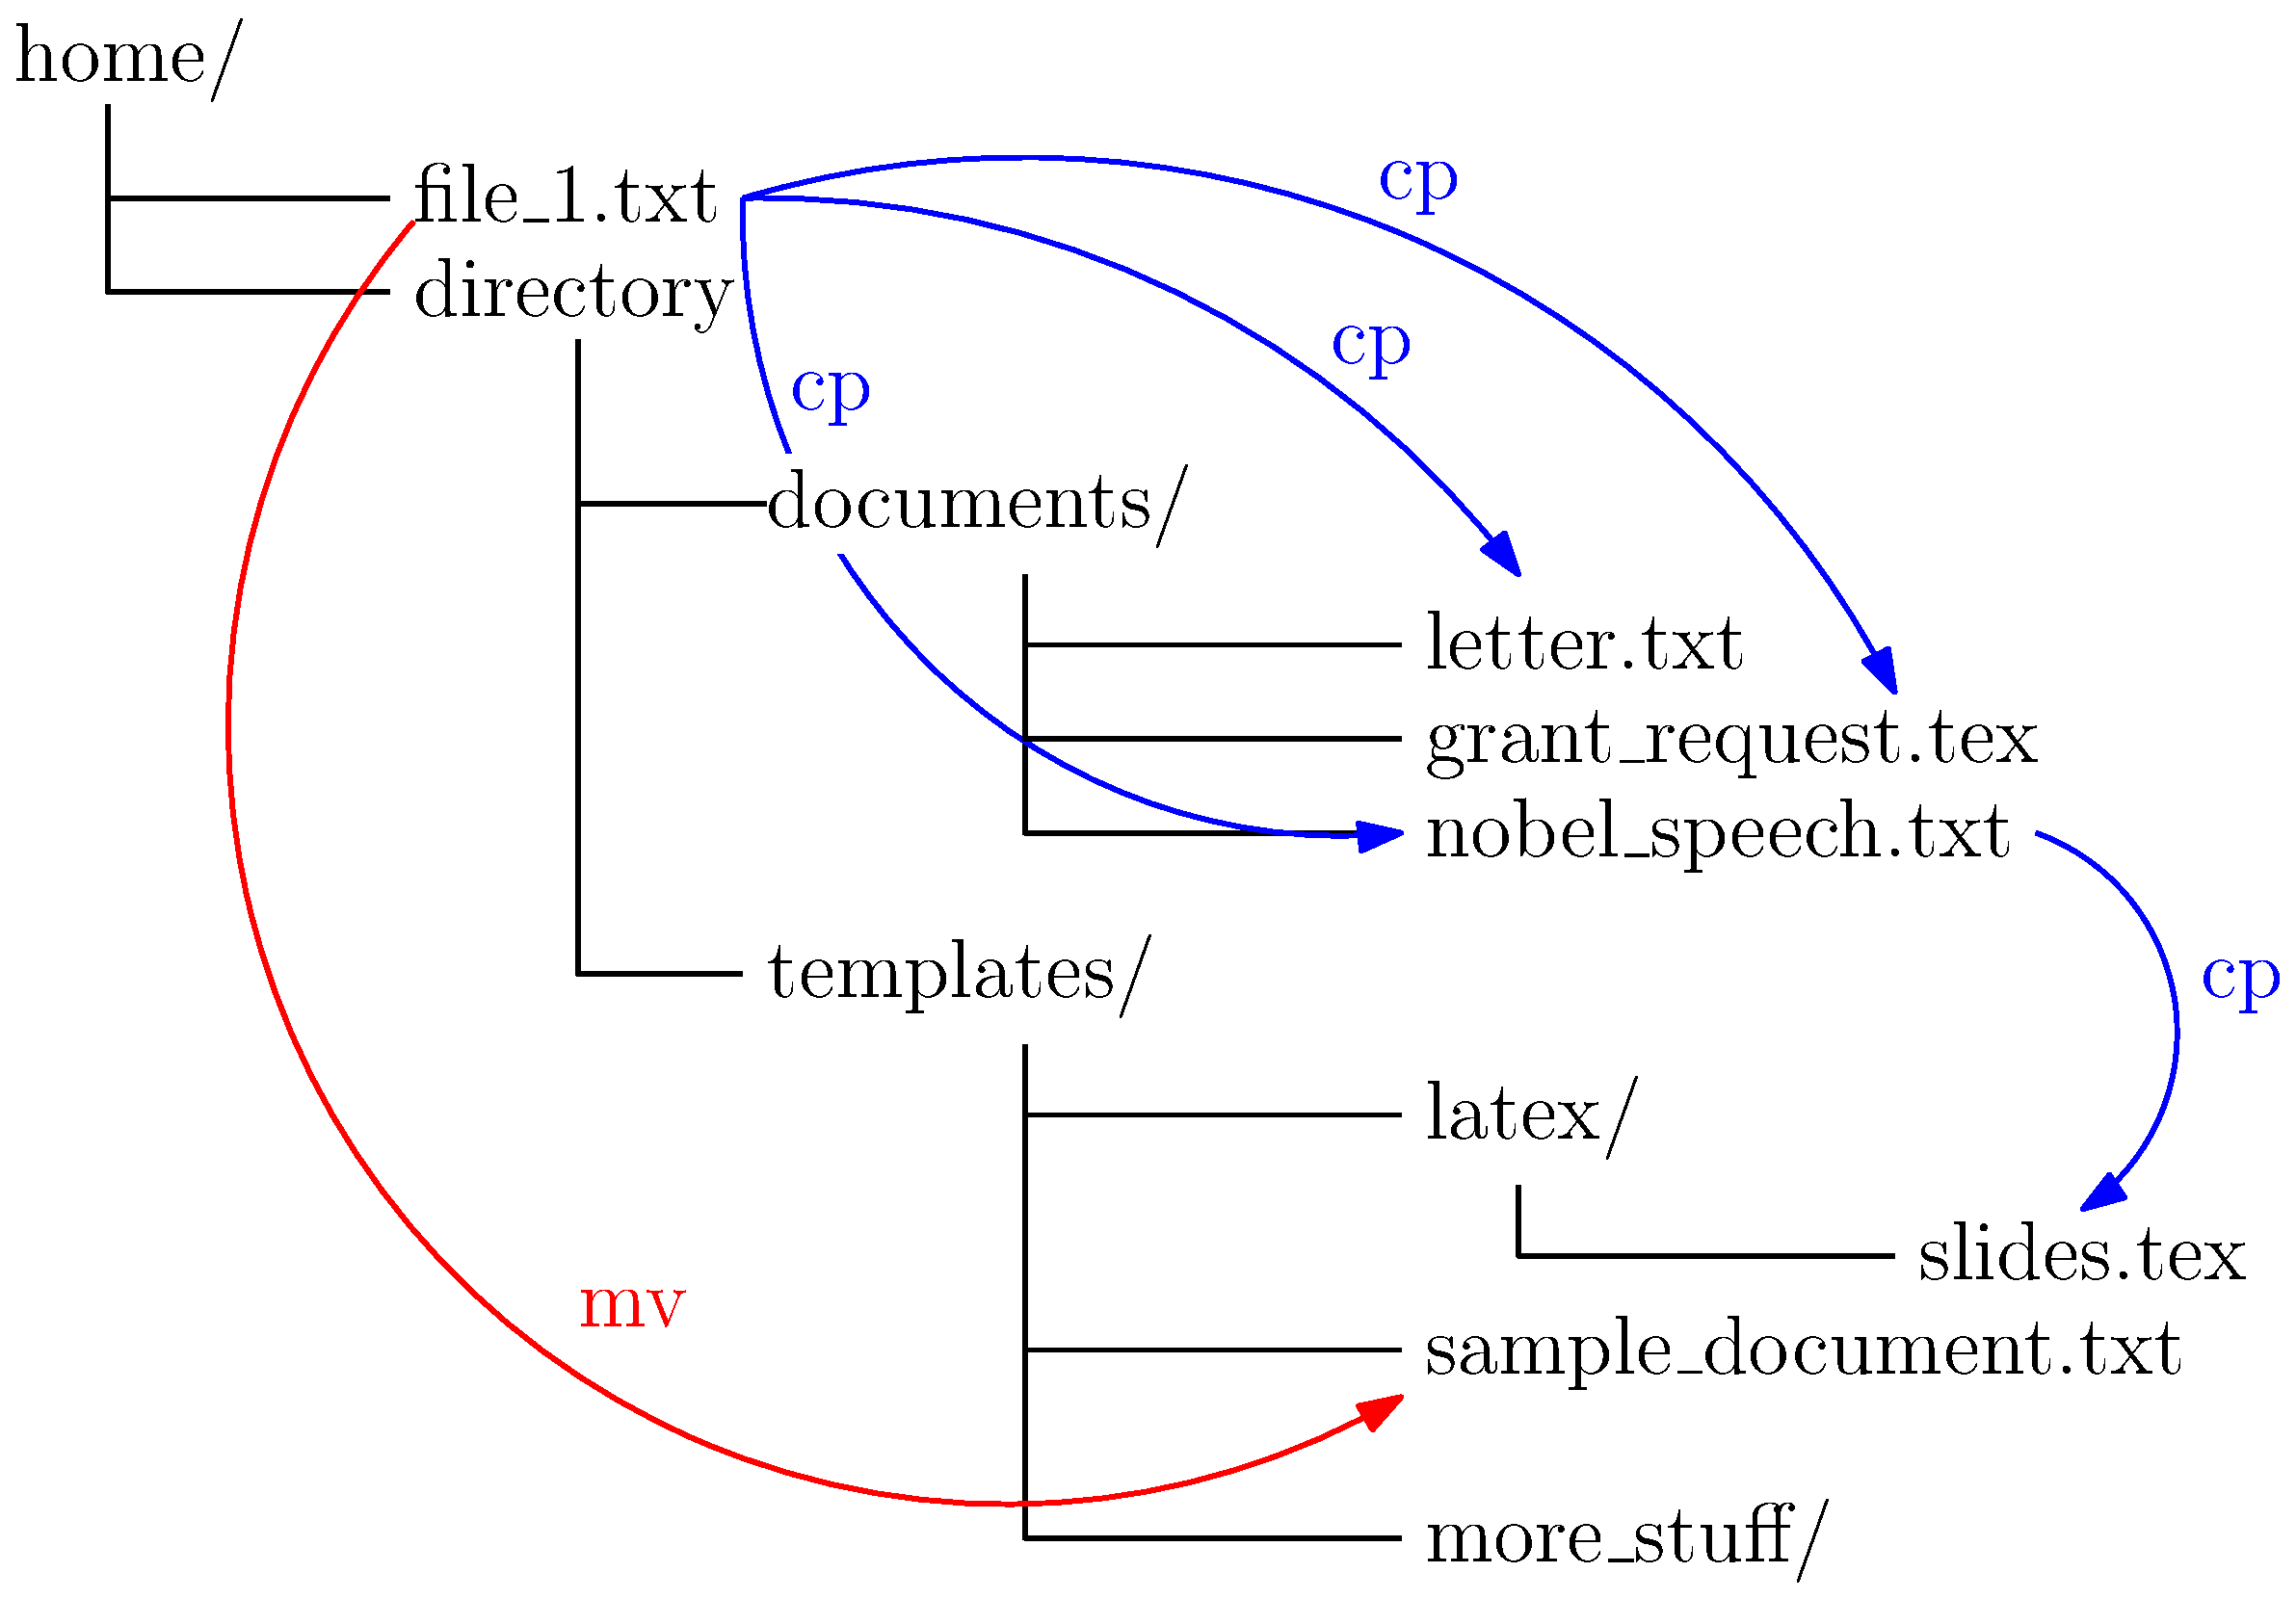
\includegraphics[width=0.77\textwidth]{pics/ex_2.eps}
    \end{center}

    Then, using \code{find}, show the location of all \code{.tex} files
  \end{center}
\end{frame}


\end{document}

%vim: tabstop=8 expandtab shiftwidth=2 softtabstop=2 spell spelllang=en_uk
